\documentclass[fr]{../../../../../../eplexam}
\usepackage{../../../../../../eplunits}
\usepackage{circuitikz}

\hypertitle{Signaux et syst\`emes}{4}{FSAB}{1106}{2015}{Janvier}
{Alexis Clarembeau\and Simon Demaré \and Louis Devillez}
{Luc Vandendorpe et Vincent Wertz}

\section{Question 1: LV1}
Considérons le filtre RLC passif de la \textsc{Figure \ref{RLC}}. On s'intéresse à la relation qu'il y a entre tension de source $x(t)$ et la tension aux bornes de l'inductance $L$, notée $y(t) = v_L(t)$

Pour rappel, les courants $i_C(t)$ et $i_L(t)$ dans la capacité $C$ et l'inductance $L$ sont respectivement donnés par:
$$i_C(t) = C \cfrac{dv_C(t)}{dt} $$
$$v_L(t) = L \cfrac{di_L(t)}{dt}$$
où $v_C(t)$ et $v_L(t)$ désignent les tensions aux bornes de la capacité et de l'inductance.
\begin{figure}[!ht]
	\centering
	\begin{circuitikz}[american]
		\draw (0,0) to[V=$x(t)$] (0,2) to[R=$R$] (2,2) to [L=$L$](4,2) to[C=$C$] (4,0) --(0,0);
	\end{circuitikz}
	\caption{Filtre RLC série}
	\label{RLC}
\end{figure}
L'équation différentielle qui lie $x(t)$ et $y(t)$ est donnée par
$$LC \frac{d^{2}y(t)}{dt^{2}}+RC\frac{dy(t)}{dt}+ y =LC\frac{d^2x(t)}{dt^2}$$
\begin{itemize}
	\item Calculez la réponse en fréquence du système
	\item Calculer la réponse impulsionnelle de ce système pour le jeu de paramètre suivants: $L = \SI{5}{mH}$, $C=\SI{100}{\micro F}$ et $H = \SI{15}{\ohm}$
	\item Dessinez le diagramme de Bode de ce système (module UNIQUEMENT de la fonction de transfert) pour les même paramètres
	\item Si l'on introduit dans le système un signal d'entrée donné par $x(t) = \cos(\omega_0t+\phi_0) +0.1\sin(\omega_1t + \phi_1)$, qu'obtient-on comme signal de sortie, $y(t)$?
\end{itemize}

\begin{solution}
	\begin{itemize}
		\item Fonction de transfert 
	$$H(jw) = \cfrac{LC(j\omega)^2}{LC(j\omega)^2+RC(j\omega)+1} $$
		\item Réponse impulsionnelle 
	$$H(jw) = \cfrac{0.5*10^{-6}(j\omega)^2}{0.5*10^{-6}(j\omega)^2+15*10^{-4}(j\omega)+1} = 1 + \frac{-3000j\omega - 2*10^6}{(j\omega+2000)(j\omega+1000)} $$
	$$H(j\omega) = 1 - \frac{4000}{j\omega + 2000} + \frac{1000}{j\omega +1000} $$
	$$y(t) = \delta(t)  + (1000e^{-1000t}- 4000e^{-2000t})u(t)$$
	
	\item diagramme de bode 
		$$H(jw) = \cfrac{(j\omega)^2}{(j\omega+2000)(j\omega+1000)} = \cfrac{(j\omega / \sqrt{2}*10^3)^2}{(j\omega/2*10^3+1)(j\omega/10^3+1)}  $$
	\begin{center}		
	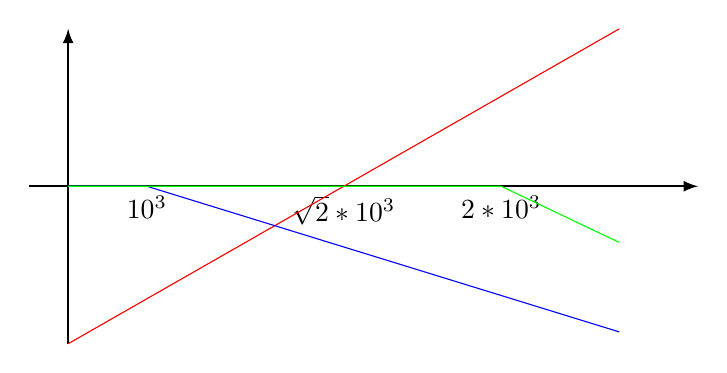
\begin{tikzpicture}
		\draw [thick,-latex] (-0.5,0) -- (8,0);
		\draw [thick,-latex] (0,-2) -- (0,2);
		\draw (1,0)node[below]{$10^3$};
		\draw (3.5,0)node[below]{$\sqrt{2}*10^3$};
		\draw (5.5,0)node[below]{$2*10^3$};
		\draw [red] (0,-2)--(7,2);
		\draw [blue] (0,0) -- (1,0) -- (7,-1.85);
		\draw [green] (0,0) -- (5.5,0) -- (7,-0.714);
	\end{tikzpicture} 
	
	\begin{tikzpicture}
	\draw [thick,-latex] (-0.5,0) -- (8,0);
	\draw [thick,-latex] (0,-2) -- (0,2);
	\draw (1,0)node[below]{$10^3$};
	\draw (3.5,0)node[below]{$\sqrt{2}*10^3$};
	\draw (5.5,0)node[below]{$2*10^3$};
	\draw [red] (0,-2)--(1,-1.42) -- (5.5,-0.19) -- (7,-0.19);
	\end{tikzpicture}
	\end{center}
	\end{itemize}
	
	\item
	$$y(t) =|H(j\omega_0)| \cos(\omega_0t+\phi_0 + \theta_0) +|H(j\omega_1)|0.1\sin(\omega_1t + \phi_1 + \theta_1)$$
	avec:
	\subitem$\theta_0 = angle(|H(j\omega_0)|)$
	\subitem $\theta_1 = angle(|H(j\omega_1)|)$
\end{solution}



\section{Question 2: LV2}
\begin{enumerate}
	\item Représentez graphiquement le résultat d’une DFT de taille 8 obtenue à partir du signal $x[n]$ dans lequel on insère chaque fois un 0 entre deux échantillons successifs ? Expliquez.
	\item On insère maintenant un zéro mais entre les échantillons successifs de la transformée de Fourier donnée sur la figure 2. On applique une IDFT de taille 8 au vecteur ainsi obtenu. Représentez graphiquement le signal obtenu dans le domaine temporel. Expliquez.
\end{enumerate}

(solution graphique: )

Attention au graduations des graphes et de (???)

\begin{solution}
Je crois que ceci passait à l'examen:
Voici la solution dans un des deux sens. Soit x, le signal de base et y, sa transformée de fourier. Soit x', le signal de base intercalé de 0. Le signal x fait une taille n et le signal x', une taille 2n.

Par application de la formule de la FFT sur x:
$$y[j] = \sum_{k=0}^{n-1} x[k] exp \left(
\frac{-2 \pi i jk }{n}
\right)$$
Et sur x' (de longueur 2n)
$$y'[j] = \sum_{k=0}^{2n-1} x'[k] exp \left(
\frac{-2 \pi i j k }{ 2n}
\right)$$
Pour toutes les valeurs de k impair, x'[k] est nul et le terme ne
contribue pas à la somme. Pour les autres valeurs, x'[k] = x[k/2]. Dans ce cas, on peut réécrire par changement de variable:
$$y'[j] = \sum_{a=0}^{n-1} x[a] exp \left(
\frac{- 2 \pi i j 2a }{2n}
\right)$$
Ou encore:
$$y'[j] = \sum_{a=0}^{n-1} x[a] exp \left(
\frac{-2 \pi i j a }{n}
\right)$$
On remarque que pour $j < n$, dans ce cas: y' = y
Pour y > n, on va poser j = n + o, afin de mettre en évidence le phénomène de duplication de la période:
$$y'[n+o] = \sum_{a=0}^{n-1} x[a] exp \left(
\frac{-2 \pi i a}{ n } (n+o)
\right)$$
Ou encore, en développant:
$$y'[n+o] = \sum_{a=0}^{n-1} x[a]
exp \left( -2 \pi j a \right)
exp \left( \frac{-2 \pi j o}{n} \right)$$
Or, on sait que $exp(-2 \pi j a ) = 1$ , car a est entier, donc:
$$y'[n+o] = y[o]$$
On a démontré ce qu'on voulait, c'est-à-dire que:
$$y'[i] = y[i]  \qquad \text{si} \quad i < n$$
$$y'[i] = y[i-n] \qquad \text{si} \quad i > n$$
Ou encore, on a périodisé une fois y.

Pour la FFT inverse, j'ai dit que c'était la même chose par réciprocité. Par contre, je ne sais pas si c'est bon. Au pire, je crois que la même démarche fonctionne aussi ici émoticône smile
\end{solution}

\section{Question3: VW1}
\begin{itemize}
	\item Calculer la sortie y(t) du système linéaire et invariant dans le temps caractérisé par la réponse impulsionnelle $h(t)= e^{-\alpha t}u(t)$ et dont l'entrée est le signal $x(t) = e^{\alpha t}u(-t)$ avec $\alpha > 0$:
	\subitem en utilisant le produit de convolution
	\subitem en utilisant la transformée de laplace
	\item Esquisser sommairement le signal y(t)
\end{itemize}

Note : cette question est la même que VW1 de Janvier 2006, disponible dans la Dropbox. Celui-ci a une solution du prof en plus (différente de celle ci-dessous), avec moins d'explications évidemment.

\begin{solution}
\subsection{Convolution}
On sait que:
$$
    y(t) = x(t)*h(t)
$$
La définition du produit de convolution donne:
$$
    y(t) = \int_{-\infty}^{\infty} x(t-\tau).h(\tau).d\tau
$$
On remplace x et h par leurs expressions:
$$
    y(t) = \int_{-\infty}^{\infty} e^{a(t-\tau)}.u(-(t-\tau)) e^{-a \tau} u(\tau).d\tau
$$
On développer l'exponentielle et sortir le terme en $a\tau$.
$$
    y(t) = \int_{-\infty}^{\infty} e^{at}.e^{-2a\tau}.u(-(t-\tau)) u(\tau).d\tau
    = e^{at} \int_{-\infty}^{\infty} e^{-2a\tau}.u(-(t-\tau)) u(\tau).d\tau
$$
L'idée est de trouver ce que signifie le produit des deux échelons: $u(\tau)$ et $u(\tau - t)$.
Pour cela, on considère deux cas: $t<0$ et $t >0$ (on peut avoir cette idée en commençant par résoudre
le laplace et en regardant l'allure de la solution).
\\

On a donc si $t > 0$: $u(\tau-t)u(\tau) = u(\tau - t)$. Ceci se vérifie si on trace les deux échelons dans un
graphe où on place en abscisse $\tau$ (attention: $\tau$ est bien la variable d'intégration, t doit être
considéré comme un paramètre).
\\

L'intégrale devient alors:
$$
    e^{at} \int_{-\infty}^{\infty} e^{-2a\tau}.u(\tau-t) d\tau
$$
Ce qui revient à faire
$$
    e^{at} \int_{\tau}^{\infty} e^{-2a\tau}.u(\tau-t) d\tau
$$
Ce qui donne:

$$
    e^{at} \left[ \frac{-1}{2a} e^{-2a\tau} \right]_{t}^{\infty}
    =
    e^{at} \cdot \left( -\frac{-1}{2a} e^{-2a t} \right)
    =
    \frac{e^{-at}}{2a}
$$
L'autre cas se situe pour $t < 0$. Dans ce cas, on remarque que  $u(\tau-t)u(\tau) = u(\tau)$.
On peut alors réduire l'intégrale d'une manière analogue:
$$
    y(t) =  e^{at} \left[ \frac{-1}{2a} e^{-2a\tau} \right]_{0}^{\infty}
    =
    e^{at} \cdot \left( -\frac{-1}{2a} e^{-2a 0} \right)
    =
    \frac{e^{at}}{2a}
$$
La solution finale est donc
$$
    \left\{
        \begin{tabular}{c}
         si $t>0$ : $y(t) = \dfrac{e^{-at}}{2a}$\\
         \\
         si $t<0$ : $y(t) = \dfrac{e^{at}}{2a}$
        \end{tabular}
    \right.
$$

\subsection{Laplace}

Ici, nous allons tenter d'obtenir la même réponse, mais cette fois-ci, avec la méthode
de Laplace.
\\

On sait que:
\[
    Y(s) = X(s).H(s)
\]
L'élément le plus compliqué est de trouver $X$ et $H$ connaissant $x$ et $h$.
On va commencer par $x(t) \to X(s)$:
\[
    x(t) = e^{at}.u(-t) = - \left[
        -e^{at}.u(-t)
    \right]
\]
La partie entre crochets se retourve dans le formulaire (attention, le a de l'équation correspond
au $-\alpha$ du formulaire):
\[
    X(s) = - \left[
        \frac{1}{s-a}
    \right]
    \qquad
    \text{ROC: }
    \qquad
    \mathbb{R}\{s\} < a
\]
Pour trouver l'expression de H, c'est encore plus simple la réponse se tire du formulaire:
\[
    h(t) = e^{-at} u(t) \rightarrow
    H(s) =
        \frac{1}{s+a}
    \qquad
    \text{ROC: }
    \qquad
    \mathbb{R}\{s\} > -a
\]
On peut alors appliquer $Y = X.H$, ce qui donne:
\begin{align*}
    Y(s) &= - \frac{1}{s-a} \cdot \frac{1}{s+a}
    \\ &= - \frac{1}{s^2 - a^2}
\end{align*}
On effectue une décomposition en fractions partielles pour obtenir la transformée inverse
et, par conséquent, l'expression temporelle:
\begin{align*}
Y(s) &= \frac{-1/2a}{s-a} + \frac{-1/(-2a)}{s+a}\\
&= \frac{-1}{2a} \cdot \frac{1}{s-a} + \frac{1}{2a} \frac{1}{s+a}
\end{align*}
Si on regarde dans la table des transformées inverse (\textbf{en regardant bien les régions de convergence}), on trouve:
\[
    \frac{-1/2a}{s-a}
    \rightarrow
    \frac{-1}{2a} \left[
        -e^{at}.u(-t)
    \right]
    \qquad
    \text{car ROC : }
    \mathbb{R} \{s\} < a
\]
\[
    \frac{1/2a}{s+a}
    \rightarrow
    \frac{1}{2a} \left[
        e^{-at}.u(t)
    \right]
    \qquad
    \text{car ROC : }
    \mathbb{R} \{s\} > -a
\]
On a alors la solution finale\footnote{ce qui est logique pour un cours de SS}:
\[
    y(t) =
    \frac{-1}{2a} \left[
        -e^{at}.u(-t)
    \right] +
    \frac{1}{2a} \left[
        e^{-at}.u(t)
    \right]
\]
Ce qui confirme ce que l'on avait obtenu avec le produit de convolution


signal y(t):
\begin{center}
	\begin{tikzpicture}
		\draw [thick,-latex] (-4,0) -- (4,0) (0,-0.5) -- (0,2);
		\draw [domain=0:4,samples=200] plot(\x,{1.5*exp(-\x)});
		\draw [domain=-4:0,samples=200] plot(\x,{1.5*exp(\x)});
	\end{tikzpicture}
\end{center}
\end{solution}
\newpage
\section{Question 4: VW2}
On considère le système invariant dans le temps représenté par le schéma-bloc suivant:
\begin{center}
	\begin{tikzpicture}
		\draw [thick,-latex](-1,0)node[left]{x} -- (-0.2,0);
		\draw (0,0)circle(0.2);
		\draw (-0.25,0)node[above]{+};
		\draw [thick,-latex] (0.2,0) -- (1,0) ;
		\draw (1,0.5) rectangle (2,-0.5);
		\draw (1.5,0) node[]{$\cfrac{1}{s+4}$};
		\draw [thick,-latex] (2,0) -- (2.8,0);
		\draw (2.7,0) node[above]{+};
		\draw [thick,-latex](2.5,0) -- (2.5,-1.5) -- (2,-1.5);
		\draw (2,-2) rectangle (1,-1);
		\draw (1.5,-1.5) node[]{$\cfrac{1}{s+2}$};
		\draw [thick,-latex] (1,-1.5) -- (0,-1.5) -- (0,-0.2);
		\draw (-0,-0.3) node[left]{-};
		\draw (3,0) circle(0.2);
		\draw [thick,-latex] (0,-1.5) -- (0,-2.5) -- (3,-2.5) -- (3,-0.2);
		\draw (3,-0.3)node[left]{-};
		\draw [thick,-latex](3.2,0) -- (4,0);
		\draw (4,-0.5) rectangle (5,0.5);
		\draw (4.5,0)node[]{$\cfrac{1}{s+K}$};
		\draw [thick,-latex](5,0) -- (5.5,0) -- (5.5,-1.05);
		\draw (5.5,-0.95)node[left]{+};
		\draw [thick,-latex](3,-2.5) -- (4,-2.5);
		\draw (4,-2) rectangle(5,-3);
		\draw (4.5,-2.5)node[]{$\frac{-1}{2}$};
		\draw [thick,-latex](5,-2.5) -- (5.5, -2.5) -- (5.5,-1.45);
		\draw (5.5,-1.55) node[left]{+};
		\draw (5.5,-1.25) circle(0.2);
		\draw [thick,-latex](5.7,-1.25) -- (6.5,-1.25)node[right]{y};
	\end{tikzpicture}
\end{center}
\begin{itemize}
	\item
	\subitem Donner une représentation d'état de ce système
	\subitem Calculez la fonction de transfert du système
	\subitem Expliquer en quelques lignes les concepts de stabilité interne et de stabilité BIBO
	\item Pour $K=1$
	\subitem Étudier la stabilité interne
	\subitem Étudier la stabilité BIBO
	\subitem Étudier la commandabilité du système
	\item Pour $K=-2$
	\subitem Étudier la stabilité BIBO
	\subitem Sans effectuer de calcul supplémentaire, que pouvez-vous dire de la commandabilité et de l'observabilité du système ?
\end{itemize}
Note : cette question est la même que VW2 d'août 2012 ainsi que janvier 2006. Celui de janvier 2006 a même une solution du prof.

\begin{solution}
	\begin{itemize}
		\item Représentation d'état:	$$
		\begin{bmatrix}
		\dot q_1(t)\\
		\dot q_2(t)\\
		\dot q_3(t)\\
		\end{bmatrix}=
		\begin{bmatrix}
		-4&-1&0\\
		1&-2&0\\
		1&-1&-K
		\end{bmatrix}
		\begin{bmatrix}
		q_1(t)\\
		q_2(t)\\
		q_3(t)
		\end{bmatrix}
		+
		\begin{bmatrix}
		1\\
		0\\
		0
		\end{bmatrix}
		x(t)$$
		$$
		y(t)=
		\begin{bmatrix}
		0&-1/2&1
		\end{bmatrix}
		\begin{bmatrix}
		q_1(t)\\
		q_2(t)\\
		q_3(t)
		\end{bmatrix}
		+
		\begin{bmatrix}
		0
		\end{bmatrix}
		x(t)$$
		
		\item Fonction de transfert:
		$$H(s)= C(sI-A)^{-1} + D$$
		
		$$(sI-A)=
		\begin{bmatrix}
		s+4&1&0\\
		-1&s+2&0\\
		-1&1&s+K
		\end{bmatrix}
		$$
		\[(sI-A)^{-1}=
		\begin{bmatrix}
		\ldots&\ldots&\ldots\\
		s+K&\ldots&\ldots\\
		s+1&\ldots&\ldots
		\end{bmatrix} \cdot \frac{1}{(s+K)((s+4)(s+2)+1)}
		\]
		\[ H(s) = \frac{s-K+2}{2(s+K)((s+4)(s+2)+1)} \]
		
	\item Un système est stable (interne) si un bruit proche de 0 va toujours se tasser pour toutes les états. C'est représenté par $\forall i$ $\Re(\lambda_i) < 0$
	
	Un système est BIBO stable si la partie observable et commandable est stable c'est à dire $\forall i$ $\Re(d_i) < 0$
	
	\item $K =1$
	\[ H(s) = \frac{s+1}{2(s+1)((s+4)(s+2)+1)}= \frac{s+1}{2(s+1)(s+3)^2} \]
	Tout les $\lambda_i$ sont négatifs, le système est asymptotiquement stable. Tout les pôles sont négatifs, le système est BIBO stable.
	
	\[
	\begin{bmatrix}
	B&AB&A^2B
	\end{bmatrix} 
	=
	\begin{bmatrix}
	 1&-4&17\\
	 0&1&-6\\
	 0&1&-6
	\end{bmatrix}\]
	On a donc une perte de commandabilité
	
	\item K = -2
	\[ H(s) = \frac{s+4}{2(s-2)(s+3)^2}\]
	Nous avons une valeur propre qui est aussi un pôle a gauche de l'axe complexe, le système est donc instable (interne et bibo)
	
	La fonction de transfert possède 3 pôles, il n'y a donc pas de perte d'observabilité ou de commandabilité
	
	\end{itemize}
\end{solution}

\end{document}
